\RequirePackage[T1]{fontenc}
\documentclass[10pt,journal,letterpaper]{IEEEtran}
\usepackage{amsmath,amssymb,amsthm,booktabs,array,microtype}
\usepackage[hidelinks]{hyperref}
\usepackage{fancyhdr,tikz,graphicx}
\usetikzlibrary{arrows.meta}
\hypersetup{pdftitle={Diskless Viewstamped Replication with Unbounded Crash-Stop Reincarnation --- Addendum},pdfauthor={Simon Massey}}
\newcommand{\paperrevision}{RESEARCH CHECKPOINT --- 11 SEPTEMBER 2026}
\newcommand{\paperversion}{ADDENDUM}
\IfFileExists{version.tex}{\input{version.tex}}{}
\pagestyle{fancy}
\fancyhf{}
\fancyhead[R]{\footnotesize\thepage}
\fancyfoot[C]{\scriptsize\paperrevision\ --- \paperversion}
\renewcommand{\headrulewidth}{0pt}
\setlength{\emergencystretch}{1em}
\raggedbottom
\newtheorem{theorem}{Theorem}
\newtheorem{lemma}{Lemma}
\newtheorem{definition}{Definition}
\newtheorem{proposition}{Proposition}
\newtheorem{remark}{Remark}
\newtheorem{example}{Example}
\newcommand{\systemname}{uVRR}
\newcommand{\QI}{\mathcal{Q}^{\mathrm I}}
\newcommand{\QII}{\mathcal{Q}^{\mathrm {II}}}
\newcommand{\code}[1]{\texttt{#1}}
\title{Diskless Viewstamped Replication with Unbounded Crash-Stop Reincarnation\\--- Addendum: proof ladder, weighted reconfiguration and the operator solver}
\author{Simon Massey\thanks{Author draft. Correspondence: simon.massey@stenographer.cloud.}}
\begin{document}
\maketitle
\thispagestyle{fancy}

\begin{abstract}
This document is an addendum to \emph{Diskless Viewstamped Replication with
Unbounded Crash-Stop Reincarnation}; the parent paper's abstract and keywords
are not repeated here. The addendum contributes what the paper does not
contain: the fuse transport with its telescoping theorem and the Lamport
induction it instantiates; the phantom-slot construction for phase one of a
five-node reincarnation; and the notational appendices for weighted
reconfiguration, the casting-vote completion with fresh identities, and the
operator solver. The parent paper supplies the method, the five-voter
schedule and the agreement result; nothing here modifies them. A companion
addendum, \emph{Experimental results}, reports the measured findings.
\end{abstract}

\section{Three voters: both transitions, then Fuse}\label{sec:fuse}
This proof ladder starts with the smallest replacement. Let the identities be
$(o,\ell,a,r)$: the retired process, surviving leader, other survivor and fresh
replacement. The complete two-transition schedule is
\[
 (1,1,1,0)\longrightarrow(0,1,1,0)\longrightarrow(0,1,1,1).
\]
The commands that install a configuration are decided under the configuration
governing their slots. For clarity, the calculations below check every row,
including the final row governing subsequent commands; this also covers either
side of each boundary.

\subsection{The base case and the second transition}
For $w:N\to\mathbb N$, write $T(w)=\sum_{n\in N}w(n)$ and
$M_w(R)=\sum_{n\in R}w(n)$. A strict majority satisfies $2M_w(R)>T(w)$.
At the first boundary any old quorum contains two of $o,\ell,a$, while every
intermediate quorum contains both $\ell,a$. Hence they meet. At the second
boundary every intermediate quorum contains $\ell,a$, and any final quorum
contains two of $\ell,a,r$. Hence they meet too. This proves the cross-era
intersection obligation for both transitions, not just the final one.

For the response set $R=\{\ell,a\}$, the masses are $2,2,2$ and the totals
are $3,2,3$. Thus exactly the same two responding identities are a majority
throughout. Adding the replacement's acknowledgement cannot invalidate that
fact. Abstract singleton-intersection witnesses are
$\{o,\ell\}\cap\{\ell,a\}=\{\ell\}$ at the first boundary and
$\{\ell,a\}\cap\{\ell,r\}=\{\ell\}$ at the second.
These geometric witnesses and the responding quorum serve different purposes:
the fused decision certificate uses $\{\ell,a\}$ and does not ask the retired
identity to reply. The existing module \path{ReincarnationThree.lean} records
both intersections and both casting witnesses.

\subsection{What a fused acknowledgement certifies}
Fuse carries a shared header, a count, and the ordered commands for consecutive
slots. FuseOk carries the individual slot acknowledgements; CommitBatch carries
the individual commits. None of these needs a range encoding. Logical slots,
configuration boundaries and their quorum families remain distinct.

Let $F=(b,s,[c_0,\ldots,c_{k-1}])$. An acknowledgement of $F$ certifies that
the sender accepted every specified command at ballot $b$ and its specified
slot. The leader matches the ballot, first slot, count and slot contents to its
pending envelope, counts each identity once, and checks its own eligibility
when adding its own acknowledgement. Let $R$ be that set of acknowledgers.
Then one collection of replies gives acceptance evidence at every packed slot.
It gives decision evidence at slot $i$ precisely when $R\in\QII_i$.

\begin{theorem}[Fuse telescoping]\label{thm:fuse}
Suppose the certified schedule preserves the invariant $R\in\QII_i$ at each
step, the first slot has $R\in\QII_0$, and every member of $R$ acknowledges
all the packed slots. Every packed slot has a phase-two decision certificate.
If the expanded history satisfies Turner's protocol invariants, the ordinary
era-based agreement theorem applies to each certificate.
\end{theorem}
\begin{proof}
Induct on the slot index. The base is the first quorum. Preservation gives
$R\in\QII_{i+1}$ from $R\in\QII_i$. The fused acknowledgements supply every
acceptance required by that quorum at slot $i+1$. Thus every slot has both a
quorum and its acceptance evidence. Expanding the envelope into those logical
events leaves the evidence unchanged; the existing agreement theorem supplies
uniqueness under its history assumptions. In-order application then advances
the committed prefix through the schedule.
\end{proof}
For three voters, the masses above discharge preservation for both steps.
The leader can collect one FuseOk from $a$, complete its own all-slot
acceptance, and issue the two commits in one CommitBatch. This is one successful
request--reply round followed by commit notification, provided the envelope's
acceptance preconditions are already established.

\section{Five voters and arbitrary solver schedules}\label{sec:fuse-five}
\subsection{The first and second transitions}
For the complete six-transition weighted replacement, let $R$ contain any
three surviving original voters and exclude $o$. The initial total is $5$ and
$M(R)=3$. Doubling gives total $10$ and mass $6$: the first boundary preserves
every quorum exactly. Introducing the replacement's unit vote gives total $11$
and mass at least $6$. The strict inequality $12>11$ proves the second
boundary's responding-quorum condition explicitly.

The remaining rows have totals $10,9,10,5$ and response masses at least
$6,6,6,3$. Each inequality stays strict. These numbers cover the full schedule
with doubling and halving, not the shorter five-voter specialisation in
\path{ReincarnationSafety.lean}. Any larger initial responding quorum excluding
the retired identity contains such a triple and therefore also qualifies.
Theorem~\ref{thm:fuse} now telescopes the same replies across all six
transitions. The ordinary cross-era intersections follow from exact scaling
at the ends and the four unit changes between them. There is no need to list
another five-voter replacement table here.

\subsection{The solver's induction invariant}
For arbitrary endpoints, use a response set $R$ that is a strict majority at
both endpoints. Define its margin $\mu_w(R)=2M_w(R)-T(w)$. The constructive
path first decreases coordinates outside $R$, then increases coordinates
inside $R$, moving only towards their targets. These edits increase the
margin. It then decreases coordinates inside $R$ and increases coordinates
outside $R$ towards their targets. Throughout these latter phases the margin
is at least the strictly positive final margin. Thus $\mu_w(R)>0$ everywhere.
Each unit edit also preserves cross-era intersection; exact scaling preserves
quorum families. Zero-weight membership edits have no effect on either proof.

This supplies a useful runtime certificate: compute the path with $R$ as the
availability set, certify the preserved margin, and use the same fused replies
at every slot. The existing operator solver and its general reachability proof
provide the construction; a Fuse integration must retain its response-set
certificate. Merely knowing that some available majority exists in each row
does not establish that every subset which replied first qualifies in all rows.
If only a larger available set $L$ was certified, the leader can use per-slot
quorum accounting on the packed acknowledgements, or wait for a response set
which satisfies the common certificate. Neither requires another wire round
when those responses arrive in the original round.

The necessity is visible in the proposed equal-total swap
$(1,2,1,2)\to(2,1,2,1)$. The response set $\{B,D\}$ has mass $4$ initially
and $2$ finally, with total $6$ at both endpoints. The same replies cannot be
counted as a final majority. Even expanding the swap into legal unit edits
does not alter that endpoint calculation. This is a negative control for the
certificate, not an obstacle to solving the reconfiguration using a suitable
common response set or successive certificates. Phantom identities remain
available for the overlap construction in Appendix~\ref{app:solver}; an
identity which sends no acknowledgement contributes no acceptance evidence.

\section{The atomicity and agreement obligations}\label{sec:fuse-refinement}
The useful state-space reduction is local: one receiver either refuses the
envelope or acknowledges its entire accepted sequence. It removes network
loss between the commands inside that envelope. Different recipients may
still receive different envelopes, and a leader may change while replies or
commits are in flight. The existing agreement proof covers such histories
when its invariants hold.

An indivisible datagram does not itself make execution of the receiver's
handler indivisible. The refinement obligation is therefore to validate the
whole fold before exposing its effects, acknowledge only after all accepts
are recorded, and ensure that interruption before acknowledgement leaves a
state admitted by the ordinary recovery or crash-stop-reincarnation model.
Checksums establish neither a transaction over memory nor a journal
transaction. Under an atomic handler model, expansion is a finite sequence of
ordinary accept actions with no intervening local action. Under a finer model,
its unacknowledged prefixes must also refine ordinary accept histories.

The induction for local acceptance needs its own invariant: the next slot is
consecutive; every command is legal in the accumulated configuration; the
promise still permits its ballot; and the slot's era permits that proposal.
A certified sequence plus preservation of these guards proves that accepting
the first permits accepting the rest. A shared header can hoist repeated
fields out of the wire encoding; it cannot discharge a changing era guard.
In particular, Turner's multi-era argument includes phase-one and value
selection obligations. A Phase2-only envelope must inherit those obligations
from established state or prove the corresponding refinement; the quorum
telescoping theorem alone does not perform phase one.

Concretely, the current ordinary accept path in
\path{src/replica/normal.rs} requires the entry era to equal the ballot era
or its successor. If a shared ballot has era $e$ and expanded entries are
assigned eras $e,e+1,\ldots,e+k$ against that one ballot, this guard implies
$k\leq1$; \path{Fuse.same_ballot_era_guard} checks that arithmetic in Lean.
That is the degenerate reading, not the envelope's. Under the atomic handler
model above, the fold evaluates each payload against the in-memory
configuration the preceding payloads established: payload $i{+}1$'s era
guard is judged in the era payload $i$'s commit folded, exactly as though
the payloads had arrived as separate datagrams with no intervening network.
The entry eras are therefore per-payload facts of the fold, discharged in
order, and the era the header carries disciplines the first payload alone.
Phase-one authority for every packed slot is the header ballot itself:
Lamport's leader executes phase one once for all future instances at the
same proposal number~\cite{fuse-paxos}, which is the induction the
telescoping theorem records.

The proof dependencies are consequently:
\[
\begin{gathered}
\text{legal schedule + preserved response quorum}\\
{}+\text{ all-slot acceptance certificate}\\
\Longrightarrow\text{ decision certificates for all slots};\\
\text{certificates + era history invariants}\\
\Longrightarrow\text{ agreement under reconfiguration}.
\end{gathered}
\]
This is the precise sense in which proving a base case and a preservation rule
replaces a separate proof for every schedule length. It does not assume the
inductive step merely because the first case succeeds.

\subsection{Prior art and executable evidence}
Lamport states the same induction as ``A newly chosen leader executes phase 1 for
infinitely many instances of the consensus algorithm \ldots\ Using the same
proposal number for all instances''~\cite{fuse-paxos}, where the ballot $b$ of a
standard message is defined to apply to all future slots until the leader is
interrupted. The fuse telescoping theorem is the same inductive logic in that the
fuse header ballot number is both a Phase~1 and Phase~2 for all commands in the
fused batch. As the messages are processed as a slab they cannot be interrupted.
Turner supplies the era-history conditions and the weighted reconfiguration
setting~\cite{turner}. The present
telescoping argument combines those obligations with a common response set;
it does not attribute a datagram-atomicity theorem to either source.

The standard-library Python checker
\path{research/weighted-reachability/check_fuse.py} enumerates all identity
subsets, including zero-weight identities. It checks both three-voter
boundaries (64 qualifying cross-quorum pairs), all six five-voter boundaries
(5,760 pairs), and every initial quorum excluding the retired identity
(respectively 2 and 10 sets, counting inclusion of the replacement).
It also checks 29,690 ordered endpoint/response-set combinations for all four
identity profiles in $\{0,1,2\}^4$, covering 99,352 unit edges of the monotone
construction. The equal-total swap is a required negative control. Its output
is \path{research/weighted-reachability/generated/fuse-summary.json}.

These are exhaustive statements about their finite domains. The inductive
argument supplies arbitrary finite schedule length. Lean checks the formal
implication and its stated hypotheses; property tests check the implementation
of packing, validation and commit application. TLA+ can model envelope delivery
as one receiver action after the refinement obligation is discharged.
Maelstrom remains useful for implementation faults involving replies, client
histories, recovery and networking. None of these tools needs to re-prove a
finite arithmetic domain already exhausted by an independent checker, but
each must test the layer for which it supplies evidence.

To replay the arithmetic from the repository root, run \code{python3} on
\path{research/weighted-reachability/check_fuse.py}.
The Lean module is \path{UVRR/Fuse.lean}; its proof
generation and kernel-check evidence are recorded beside the proof ladder.

\section{A phantom slot: phase one of a five-node
reincarnation}\label{sec:phantom}
The telescoping certificate of Section~\ref{sec:fuse} is stated against quorum
families, not against the lifecycle that changes them. This section records the
first phase of a five-node reincarnation in \systemname{}: the initial
configuration with its preallocated phantom slot, the serving leader's declared
overlap, the crash, and the resurrection of the crashed identity into the
phantom slot, with the quorum arithmetic stated at each step. The later phases
--- the forced weight sequence that grants the fresh identity its vote and
retires the old one --- are named where they arise and are not written here.

\begin{definition}[Phantom slot]\label{def:phantom}
A \emph{phantom slot} is a member record of the committed configuration held at
voting weight zero: a preallocated future slot for a resurrection. A phantom
contributes no mass to any quorum; messages from it are discarded by the
membership check, while messages to it are delivered.\footnote{The standby of
the reincarnation design: zero voting weight, streamed the leader's traffic,
and voting only after a committed increment grants it weight.}
\end{definition}

Let $N=\{n_1,\dotsc,n_6\}$ carry the committed weights $(1,1,1,1,1,0)$: five
unit voters $n_1,\dotsc,n_5$ and $n_6$ a phantom slot, preallocated so that a
resurrection finds its record ready, and drawn from the start so that the
figures can name it. The total is $T=5$ and the old view's quorum family is the
strict-majority family of the weights: $R$ qualifies exactly when
$2M_w(R)>5$, that is when $M_w(R)\geq3$ --- a majority of five is three. The
phantom's zero weight decides no membership: $M_w(R\cup\{n_6\})=M_w(R)$ for
every $R$.

The leader is $n_3$, and it declares its overlap as in
Figure~\ref{fig:overlap}: an active decision quorum $q=\{n_1,n_2,n_3\}$ of the
old view and a prospective phase-one quorum $q'=\{n_3,n_4,n_5\}$ for the next,
meeting the casting-vote condition $q\cap q'=\{n_3\}$ of~\eqref{eq:leader}.
While it collects the promises of $q'\setminus\{n_3\}$, the leader services the
current view: its beacon proposal and its own vote are carried forward across
the preparation.\footnote{``Beacon proposal'' is the operator's term for the
leader's continued proposal traffic at the current ballot while its own promise
is withheld; the declared overlap is that proposal together with the leader's
vote.}

Then $n_5$ crashes. A crash changes no weight: only committed configuration
commands do. The committed configuration stays $(1,1,1,1,1,0)$, so the old
view's quorum family is unchanged by the crash; what changes is availability.
Four unit voters survive against one unavailable: the available mass is $A=4$,
the unavailable mass is $D=1$, and $A>D$.

The crashed process restarts dirty and bumps its own identity: it reincarnates
as $n_6=n_5{+}1$, the own-id-increments rule of the reincarnation wire
(\path{Reincarnation.bump} in the Lean development), and announces the pair
$(n_5,n_6)$ to all; only the leader responds. The fresh identity lands in the
preallocated phantom slot --- which is why the slot was preallocated --- and
lights it up as a live standby of weight zero. Until a committed membership
change assigns it weight, $n_6$ votes nowhere.

\begin{proposition}[Phase-one quorum arithmetic]\label{prop:phantom}
Throughout phase one the configured total stays $T=5$ and the majority
threshold stays $3$: the crash removes availability, not weight, and the
phantom adds zero. Explicitly: the old view's quorum family is
$\{R\subseteq N:2M_w(R)>5\}$ computed on $w=(1,1,1,1,1,0)$; the live mass is
$5-1+0=4$, a majority of five minus the crashed vote plus the phantom's zero
weight, and $2\cdot4>5$; any three of the four survivors form a quorum, since
$2\cdot3=6>5$; and the declared overlap pair still meets in exactly
$\{n_3\}$.
\end{proposition}
\begin{proof}
Each clause is arithmetic on the displayed $w$. The family clause restates the
strict-majority definition; a crash edits no weight, so the family is
unaffected. The phantom clause is $w(n_6)=0$. The live-mass clause sums the
four surviving unit weights; the strict inequality $2M>T$ holds at $M=4$ and at
$M=3$. The overlap clause is set intersection:
$\{n_1,n_2,n_3\}\cap\{n_3,n_4,n_5\}=\{n_3\}$. Any other prepare quorum drawn
from the survivors still meets every old decision quorum, because two subsets
each of mass at least $3$ out of a total of $5$ must share a member.
\end{proof}

\begin{figure*}[t]
\centering
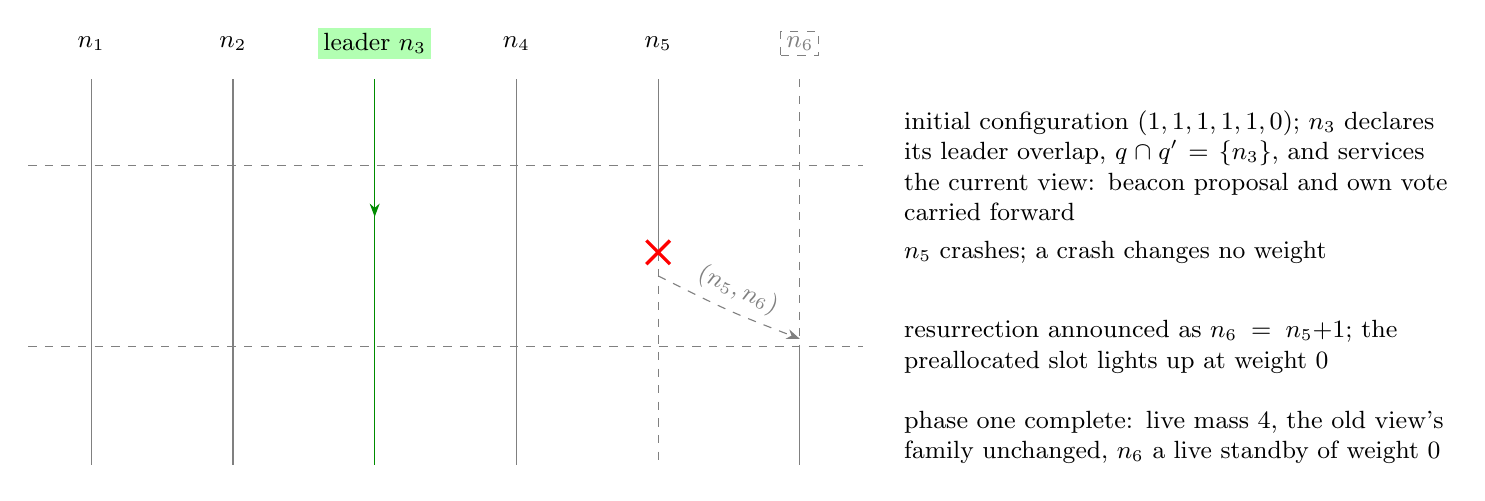
\begin{tikzpicture}[x=1cm,y=1cm,>=Stealth,font=\small]
\node at (0,0.45) {$n_1$};
\node at (1.8,0.45) {$n_2$};
\node[fill=green!30,inner sep=2pt] at (3.6,0.45) {leader $n_3$};
\node at (5.4,0.45) {$n_4$};
\node at (7.2,0.45) {$n_5$};
\node[draw,gray,dashed,inner sep=2pt] at (9,0.45) {$n_6$};
\draw[gray] (0,0)--(0,-4.9);
\draw[gray] (1.8,0)--(1.8,-4.9);
\draw[green!55!black] (3.6,0)--(3.6,-4.9);
\draw[gray] (5.4,0)--(5.4,-4.9);
\draw[gray] (7.2,0)--(7.2,-2.2);
\draw[gray,dashed] (7.2,-2.2)--(7.2,-4.9);
\draw[gray,dashed] (9,0)--(9,-3.4);
\draw[gray] (9,-3.4)--(9,-4.9);
\draw[->,green!55!black,dashed] (3.6,-0.3)--(3.6,-1.75);
\draw[dashed,gray] (-0.8,-1.1)--(9.8,-1.1);
\node[anchor=west,align=left,text width=6.9cm] at (10.2,-1.1) {initial
configuration $(1,1,1,1,1,0)$; $n_3$ declares its leader overlap,
$q\cap q'=\{n_3\}$, and services the current view: beacon proposal and own
vote carried forward};
\draw[red,very thick] (7.05,-2.35)--(7.35,-2.05) (7.05,-2.05)--(7.35,-2.35);
\node[anchor=west,align=left,text width=6.9cm] at (10.2,-2.2) {$n_5$ crashes;
a crash changes no weight};
\draw[->,gray,dashed] (7.2,-2.5) .. controls (8.1,-2.95) .. (9,-3.3)
node[midway,above,sloped] {$(n_5,n_6)$};
\draw[dashed,gray] (-0.8,-3.4)--(9.8,-3.4);
\node[anchor=west,align=left,text width=6.9cm] at (10.2,-3.4) {resurrection
announced as $n_6=n_5{+}1$; the preallocated slot lights up at weight $0$};
\node[anchor=west,align=left,text width=6.9cm] at (10.2,-4.55) {phase one
complete: live mass $4$, the old view's family unchanged, $n_6$ a live standby
of weight $0$};
\end{tikzpicture}
\caption{Phase one of a five-node reincarnation with a preallocated phantom
slot. Six membership slots $n_1,\dotsc,n_6$; the phantom $n_6$ is drawn grey
and dashed from the start at weight $0$ and lights up when the crashed $n_5$
resurrects into it. The leader $n_3$ (filled) declares its overlap --- beacon
proposal and own vote carried forward, dashed --- and services the current view
throughout. A crash changes no weight: the configured total stays $5$ and the
majority threshold stays $3$; the live mass is $5-1+0=4$. Time runs downwards
without a scale.}
\label{fig:phantom-phase-one}
\end{figure*}

\begin{remark}[The later phases, named]\label{rem:later-phases}
Phase two is the leader's forced weight sequence over the six-slot membership
of Table~\ref{tab:weights} --- the doubling, the join and increment that grant
$n_6$ its vote, the decrements that retire $n_5$, and the halve back to unit
weights --- with the leader's memo-stream keeping the standby current
throughout. Phase three is the completion: $n_5$ leaves the membership and the
cluster returns to five unit voters, now with $n_6$ among them. Neither is
written here.
\end{remark}


\section{Witness acquisition: the joiner learns the era before it
participates}\label{sec:witness}

The phantom-slot analysis of \S\ref{sec:fuse} exposed the failure shape this
section removes: a node whose engine starts uninformed receives traffic from
an era it cannot classify, and the one-era recovery gate drops what it
cannot span. The fix is not a wider gate. A node that is not a member of the
cluster has no business guessing an era at all; it learns the era first,
from the cluster, and only then lets its engine see a message. The whole
mechanism is a wrapper --- the \emph{find-the-cluster guard} --- around the
unmodified node engine, plus a \emph{witness list} held at every node and
acted on by the leader. Neither touches a quorum rule.

\subsection{The find-the-cluster guard}
A server that wants to join is known to the operator and mutually
authenticated (a pre-shared key is sufficient; the channel assumption is
environmental, not protocol). It holds some files describing which nodes
were recently in the cluster. It broadcasts a join request to all of them;
it may miss the current leader, but every member answers with the pair
(era, membership) \emph{as committed locally}. Era advances only when a
committed batch is applied, so no honest response can name an era the
cluster has not committed. The guard:
\begin{enumerate}
\item adopts the maximum reported era and the membership that response
  carried --- the true era is that or something ahead of it, never behind;
\item flushes the adopted (era, membership) to durable storage whenever the
  adoption changes, so a crash during acquisition restarts from the best
  known pair rather than from blank;
\item runs its own retransmission loop until acquisition completes --- the
  first responder may be stale or partitioned, and the leader may move
  while the responses are in flight.
\end{enumerate}
The guard then hands the engine a valid (era, membership) pair. The engine
never executes the drop path that stranded the phantom-slot joiner, because
no message can now arrive from an era it has not already adopted or cannot
reach by the ordinary guards.

\subsection{The witness list}
The join request names the joiner's frontiers (blank for a reincarnated
node). \emph{Every} node that hears the request records the sender as a
\emph{witness} --- present on an operator-visible list, absent from the
voting configuration. The leader alone acts on the list:
\begin{enumerate}
\item replays the contiguous suffix of its journal from the advertised
  frontier, in order, each entry subject to the ordinary accept path's
  first-slot discipline; then the commit frontier, which never exceeds the
  highest replayed slot (commit information rides the stream exactly as
  VRR-2012 \S4.1 step~6 rides it on \textsc{Prepare});
\item copies the witness on all subsequent phase-2 traffic and commits.
  The first commit the witness folds starts its leader-timeout; it behaves
  as a passive sink that happens to be precisely up to date;
\item every node removes the witness entry when a committed batch makes the
  witness a member: delivery as both voter and witness in the window
  between the commit and the removal is covered by ingress deduplication
  by (view, slot) and merely wastes IO.
\end{enumerate}
Because the list rides at every node from the moment the gossip lands, a
successor leader resumes the stream on election without waiting for a
re-announcement: failover does not interrupt keep-up. The guard's
retransmission loop remains load-bearing as the gossip's own reliability
--- a request lost in flight is re-sent, naming the current frontiers, and
a node that missed the original learns of the joiner from the resend. A
witness that is never promoted is an append-only audit tape of everything
the cluster committed; a statically registered witness is never purged, so
the disaster-recovery sink costs exactly the stream that reincarnation
already needs, under every leader in turn.

\subsection{Safety conditions and kernel-checked content}
The construction is safe under five hypotheses, each of which is a
construction rule rather than an assumption about timing:
\begin{description}
\item[H1] Respondents report only committed (era, membership) pairs.
  Holds because era advances on commit application.
\item[H2] The guard adopts the maximum reported era with that response's
  membership.
\item[H3] The replay is the contiguous suffix from the advertised frontier,
  folded in order by the ordinary accept path. There is no
  witness-specific accept path.
\item[H4] Messages from non-members are discarded at ingress; the witness
  votes nowhere and its promises are counted nowhere.
\item[H5] The leader sends phase-2 only for views whose phase-1 completed
  on a quorum of members.
\end{description}

Under H1--H5 the following are kernel-checked in \code{UVRR/Witness.lean}
(zero external dependencies):
\begin{description}
\item[W-era-bound] The adopted era never exceeds the committed era
  (\code{adopt\_le\_of\_honest}).
\item[W-era-exact] Once the leader's response arrives, the adopted era
  equals the committed era (\code{adopt\_eq\_of\_leader}).
\item[W-replay] A journal holding exactly the frontier prefix, extended by
  the in-order contiguous suffix, reconstructs the leader's prefix:
  $\mathit{log}.k \oplus \mathit{replay}(\mathit{log},k,n) =
  \mathit{log}.n$ (\code{replay\_reconstructs}). A blank reincarnation is
  $k=0$ (\code{replay\_from\_blank}).
\item[W-promotion] The witness's committed prefix at any committed frontier
  equals the leader's committed prefix --- hence equals any member's, whose
  report is a prefix of the primary by the fixed-view invariant
  (\code{promotion\_committed\_prefix} with
  \code{NormalLog.reachable\_inv}). Promotion therefore admits a voter
  whose state is indistinguishable from a member that caught up by
  ordinary state transfer, and quorum certificates that count it rest on
  the same evidence as for any member.
\item[W-non-interference] No quorum contains the witness
  (\code{witness\_not\_in\_quorum}): quorum membership is decided by the
  configuration, and the witness is not in it.
\end{description}
Two fault controls pin the hypotheses. \code{invented\_era\_breaks\_bound}:
a report above the committed era breaks W-era-bound, so H1 is load-bearing
--- this is the failure that stranded the phantom-slot joiner, and the
guard exists precisely to make it unrepresentable at the engine.
\code{gapped\_replay\_fails}: a replay that skips an entry cannot
reconstruct the prefix, so the slot discipline of H3 is load-bearing.

\subsection{The implicit promise, and honest scope}
A leader that streams phase-2 at view $v$ to a witness is telescoping a
promise: per Lamport, a promise at ballot $b$ covers all lower ballots, so
accepting at $v$ raises the witness's promise floor to $v$ exactly as if a
\textsc{Prepare}(v) had been received first. The witness forfeits nothing
by raising the floor: its prior promises were counted in no quorum (H4),
and the leader's right to send at $v$ was earned from members (H5). This
paragraph is argued, not mechanised; it stands at the same layer of
obligation as the accept-path era guard of \S\ref{sec:fuse-refinement},
and we say so rather than imply otherwise. Authentication, the network and
the witness's timeout are environment; the durable adoption record is an
instance of the termination obligations' marker storage.


\section{Introduction}\label{sec:intro}
Oki and Liskov introduced Viewstamped Replication in 1988~\cite{vr}.
Liskov and Cowling's 2012 Viewstamped Replication Revisited (VRR) eliminated
disk writes during normal processing and view changes~\cite{vrr}.
Replication therefore retained the state needed for agreement without adding a
local disk flush to each update. The remaining difficulty was how to bring a
replica back after loss of that state.

Michael \emph{et al.} exposed a safety failure in VRR's recovery mechanism in
2016~\cite[Sec.~4.2 and Appendix~A.1]{diskless}.
A replica can send a view-change commitment, crash, and return in an older view
having forgotten the commitment.
It can then help commit an operation that a later leader loses when delayed
view-change messages arrive.
Their counterexample breaks linearizability, including when channels preserve
message order.
The authors provide a virtual stable storage construction to support diskless
crash recovery.
Their result makes the problem precise: restoring a replica's data must also
preserve the commitments made by its identity.

Unbounded Viewstamped Replication Revisited (uVRR) repairs this failure by
making a crash final for the protocol identity.
The crashed identity never resumes execution.
The process that replaces it joins under a fresh identity, receives state from
the cluster, and acquires voting authority through committed membership changes.
Messages sent before the crash remain messages of the old identity; the new
process cannot add fresh votes to that identity's history.
A cleanly stopped process can instead restart under its existing identity because
it has preserved its protocol state.
Startup fencing and clean shutdown use durable writes, keeping those writes
outside normal replication. Loss of volatile state therefore leads to replacement
of a member: crash recovery becomes crash-stop reincarnation.

Turner supplies the construction that connects this lifecycle to continued
replication~\cite{turner}.
Where the leader is the sole intersection of an active decision quorum and the
next prepare quorum, it can withhold its own promise while collecting the others.
The active quorum remains usable during that preparation; the leader completes
the handover with its own local promise.
We use this leader overlap to organise reincarnation.
For five unit-weight voters, the runtime schedule has six committed batches,
including exact doubling and halving. The simplified two-batch instantiation
retained for the concrete lifecycle theorem is stated separately in Appendix A.
Appendix B supplies a general configuration-path constructor and an abstract
casting-vote completion using fresh identities. Turner's agreement argument
supplies the basis for composing safe adjacent configuration boundaries.

Together, these ideas retain VRR's diskless normal path while giving failed
members a route back through fresh identities.
The intended setting is agreement over small amounts of metadata embedded in a
distributed application~\cite{motivation}.
Such a service can coordinate membership or advisory-lock metadata without
putting synchronous persistence on every update's critical path.
Its normal replication need not wait for a disk flush or batch updates to
amortise one.

Section~\ref{sec:method} develops the lifecycle and leader-overlap construction.
Section~\ref{sec:results} gives the five-voter schedule and its Lean proof of
per-slot agreement from the protocol's history invariants, together with the
replacement weights, exclusion of the evicted voter and identity nonreuse.
Section~\ref{sec:discussion} develops the metadata applications, and the appendix
sets out the mathematical hypotheses and verification evidence.
The name ``unbounded'' follows Turner's treatment of pipelining through
reconfiguration: agreement does not depend on a fixed bound on outstanding slots.

\section{Method}\label{sec:method}
\subsection{Processes, state and identity}
The agreement model is asynchronous and non-Byzantine. Messages may be delayed, and an old message retains the identity that issued it. Each incarnation has a logical identity distinct from its physical host. The lifecycle must ensure that an identity never produces new protocol actions after a replacement incarnation takes over.

A clean stop first quiesces protocol processing, then flushes the state required for restart, and finally records a durable stopped marker. On startup, a valid stopped marker permits the process to reload that state and enter \emph{Restarting} with the same identity. Before sending protocol messages it durably records that it is running again. This boot fence prevents a later crash from being mistaken for another clean restart. A restarting process retains its promises and accepted state, so ordinary timeout processing is permitted by the design.

Without a valid clean-stop marker, startup enters \emph{Joining} under a fresh identity. The old identity is crash-stopped. Cached state may reduce transfer work, but it provides no voting authority. The joiner asks the leader to evict the old incarnation and admit the new one; the leader can send missing state while coordinating the change. A joiner does not vote or initiate a view change. Its authority comes from the committed configuration, never from the fact that it shares a host with a former voter.

The implementation design uses replicated superblock markers and majority interpretation of valid marker copies. This paper abstracts that mechanism as correct clean-stop classification and durable identity fencing. The Lean result concerns the resulting lifecycle; it does not model the storage protocol itself.

\subsection{Quorums across eras}
An era determines the quorum families for a suffix of log slots. Write $\QI_e$ for its phase-one family and $\QII_e$ for its phase-two family. The history model requires the following within-era and adjacent-era intersections:
\begin{align}
q\cap r&\ne\varnothing
&& (q\in\QII_e,\ r\in\QI_e),\label{eq:same}\\
q\cap r&\ne\varnothing
&& (q\in\QI_e,\ r\in\QII_{e+1}).\label{eq:adjacent}
\end{align}
The direction in~\eqref{eq:adjacent} matters: the earlier phase-one quorum must meet the later decision quorum. These conditions are part of Turner's era-based agreement argument~\cite{turner}.

Our concrete schedule uses the same strict weighted-majority family for both phases. If $w_e(n)$ is a nonnegative integer weight on a finite support, a quorum $q$ satisfies
\begin{equation}
2\sum_{n\in q}w_e(n)>\sum_n w_e(n).
\label{eq:majority}
\end{equation}
The weighted proof establishes the requisite intersections when successive configurations differ by at most one unit of total absolute weight. Membership records for zero-weight nodes may change in the same batch without altering~\eqref{eq:majority}. A crash itself does not change any weight; only committed configuration commands do.

\subsection{The leader as the overlap}
Suppose a leader $\ell$ uses ballot $b$ with an active decision quorum $q$. To prepare ballot $b'>b$ for the next era, it chooses a prospective phase-one quorum $q'$ with
\begin{equation}
q\in\QII_e,\qquad q'\in\QI_{e+1},\qquad q\cap q'=\{\ell\}.
\label{eq:leader}
\end{equation}
This is Turner's casting-vote condition~\cite{turner}. The leader first sends prepare requests only to $q'\setminus\{\ell\}$. Their promises do not disable an acceptor in $q$. The leader withholds its own promise and may continue proposing at $b$, provided no other event invalidates the old ballot's guards.

After receiving those promises, the leader chooses the suffix boundary $k$ and makes its own promise locally. Phase one is then complete without another network exchange for the leader's response. Proposals at $b'$ must still obey the normal rule for preserving values reported by phase one. Figure~\ref{fig:overlap} shows the message order.

Decision quorums follow the era of the \emph{slot}, not simply the era associated with a ballot. Consequently, continuing to decide later-era slots at $b$ also requires a quorum valid for those slots. In the concrete pivot below, the active quorum is a majority in both adjoining eras.

\begin{figure*}[t]
\centering
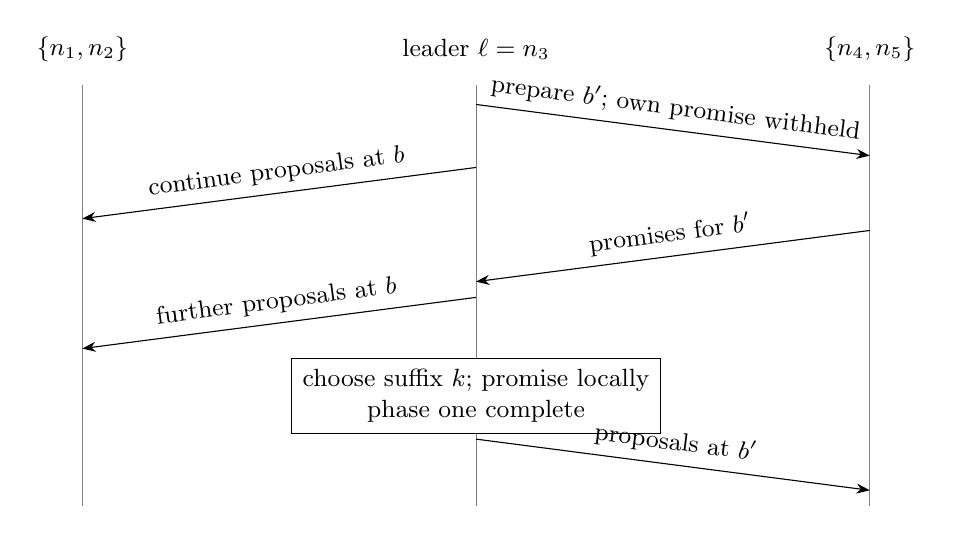
\begin{tikzpicture}[x=1cm,y=1cm,>=Stealth,font=\small]
\node at (0,0.45) {$\{n_1,n_2\}$};
\node at (5,0.45) {leader $\ell=n_3$};
\node at (10,0.45) {$\{n_4,n_5\}$};
\foreach \x in {0,5,10} {\draw[gray] (\x,0)--(\x,-5.35);}
\draw[->] (5,-0.25)--node[above,sloped]{prepare $b'$; own promise withheld}(10,-0.9);
\draw[->] (5,-1.05)--node[above,sloped]{continue proposals at $b$}(0,-1.7);
\draw[->] (10,-1.85)--node[above,sloped]{promises for $b'$}(5,-2.5);
\draw[->] (5,-2.7)--node[above,sloped]{further proposals at $b$}(0,-3.35);
\node[draw,fill=white,align=center,inner sep=4pt] at (5,-3.95) {choose suffix $k$; promise locally\\phase one complete};
\draw[->] (5,-4.5)--node[above,sloped]{proposals at $b'$}(10,-5.15);
\end{tikzpicture}
\caption{Leader overlap in the simplified Appendix A schedule at $E_1\rightarrow E_2$: $q=\{n_1,n_2,n_3\}$ and $q'=\{n_3,n_4,n_5\}$. Original schematic of Turner's casting-vote construction~\cite{turner}, specialised to the replacement schedule. Time runs downwards without a scale. Group arrows represent messages to each member; acceptance replies, state transfer and unrelated traffic are omitted.}
\label{fig:overlap}
\end{figure*}

\subsection{Replacing one of five voters}
Let $n_0$ be the failed incarnation, $n_1,\ldots,n_4$ the other original voters, and $n_5$ its fresh replacement. Table~\ref{tab:weights} gives all six committed boundaries of the five-voter weighted replacement. A join inserts the replacement at zero weight before its first increment; a leave removes the old identity after its final decrement. The three-voter unit-weight case uses two batches. These are distinct schedules, both covered by the Rust tests.

\begin{table}[t]
\centering
\caption{Full five-voter replacement: six committed batches. Zero denotes voting weight, including identities absent from membership.}
\label{tab:weights}
\small
\begin{tabular}{lrrrrrr}
\toprule
Stage & $n_0$ & $n_1$ & $n_2$ & $n_3$ & $n_4$ & $n_5$\\
\midrule
Initial & 1&1&1&1&1&0\\
Double & 2&2&2&2&2&0\\
Join, increment & 2&2&2&2&2&1\\
Decrement old & 1&2&2&2&2&1\\
Decrement, leave & 0&2&2&2&2&1\\
Increment new & 0&2&2&2&2&2\\
Halve & 0&1&1&1&1&1\\
\bottomrule
\end{tabular}
\end{table}

Each boundary preserves cross-era majority intersection by a unit change or exact scaling. Figure~1 depicts the pivot of the simplified agreement instantiation retained in Appendix~\ref{app:proof}; it is not a diagram of all six weighted boundaries. A failed witness for a particular pair of quorum sets does not establish failure of reconfiguration reachability. Appendix~\ref{app:solver} constructs paths with an available majority and shows how fresh logical identities supply an abstract singleton leader intersection. Membership weight and receipt of a protocol message remain distinct quantities.

\section{Results}\label{sec:results}
\subsection{The agreement result}
The final Lean theorem composes an era-based agreement theorem with the concrete replacement weights and an abstract identity lifecycle. Its contract assumes a well-founded total ballot order, a ballot-to-era map monotone in ballot order, the required ballot/slot era bound, and the history invariants corresponding to Turner's P2--P7~\cite{turner}. Appendix~\ref{app:proof} states the assumptions and reproduction procedure. Those invariants constrain promises, reports of prior acceptances, phase-one justification and value selection, acceptance of proposals, and quorum evidence for a chosen value. The theorem derives quorum intersection from the weight schedule.

\begin{theorem}[Five-voter replacement]\label{thm:replacement}
For a history whose phase-one and phase-two quorum families follow the simplified Table~\ref{tab:agreementweights}, assuming the ballot-order, era and history conditions above, any two values chosen for the same slot are equal. In $E_1$, both the failed identity and its replacement have zero weight; in $E_2$, the failed identity has zero weight and its replacement has unit weight. From completion of the crossing era onwards, the old identity has no voting weight in any continuation of the forced configuration run. Separately, along an identity run satisfying the formal lifecycle transitions, an identity that has been superseded by a bump is never again the current identity.
\end{theorem}

\begin{proof}
The strict-majority construction and one-unit boundaries establish the within-era and adjacent-era quorum intersections~\eqref{eq:same}--\eqref{eq:adjacent}, together with quorum nonemptiness. Instantiating the era-based agreement theorem with those families establishes equality of chosen values under the supplied history invariants. Evaluation of the concrete configurations establishes the stated weights. The eviction invariant preserves zero weight for the old identity along the forced run. The identity lifecycle transitions preserve monotonic identity growth, excluding a superseded identity from becoming current again.
\end{proof}

The leader-overlap lemmas establish that preparing members outside the active quorum preserves that quorum's guards, and that adding the leader's promise completes the prospective phase-one quorum.

\subsection{Evidence and reproduction}
The Lean 4 project is archived at repository commit \code{352b0bf}~\cite{artifact}, extended here by adding the existing eviction invariant to the final conjunction. It uses Lean~4 version~4.33.1~\cite{lean4} without Mathlib. The source directory is \path{formal/uvrr-lean/UVRR/}. The weighted intersection, era agreement, casting-vote and simplified five-voter modules supply the components of Theorem~\ref{thm:replacement}. Its final statement is \path{ReincarnationSafety.five_safe}, in \path{ReincarnationSafety.lean}, importing \path{ReincarnationAgreement.lean}.

From \code{formal/uvrr-lean}, run \code{lake build} and \code{python3 check\_axioms.py}. The checked baseline's axiom audit covers 355 declarations and permits only Lean's standard logical axioms; it rejects proof holes and custom axioms. The recorded rung-26 evidence also exercises a negative control that tries to give the replacement voting weight in $E_1$. Its failure checks that particular erroneous claim. The repository contains the proof-generation transcript; generated proof terms are checked by Lean, and the generator is not part of the trusted proof checker.

Theorem~\ref{thm:replacement} covers the simplified two-batch instantiation with its final configuration retained thereafter. Appendix~\ref{app:solver} supplies the general weighted reachability result and the runtime solver contract. The general weighted-intersection lemmas have broader scope than this instantiation.

\section{Discussion}\label{sec:discussion}
\subsection{Applications}
The intended deployment is an embedded authority for small metadata, with ordinary replication performed in memory.

\paragraph{Short-lived advisory locks and leader leases}
A replicated state machine can order acquisition, renewal and expiry decisions over a small record containing an owner, generation and expiry policy. An expiry command for an old generation must not revoke a newer grant. If a client uses ownership to control an external resource, that resource may also need to reject stale generations. A real-time leader lease additionally needs explicit clock and timing assumptions.

\paragraph{A membership authority for another algorithm}
An application whose bulk algorithm uses gossip or another weaker consistency model may still need one agreed version of cluster membership, ownership assignments or configuration changes. An embedded replicated state machine can supply that authority, while the bulk algorithm disseminates or consumes its decisions.

\paragraph{The CORFU precedent}
CORFU provides a concrete precedent for compact configuration metadata alongside a larger storage system~\cite{corfu}. Its reconfiguration is patterned after Vertical Paxos; Section 2.5 describes storage units acting as acceptors in a Paxos-like protocol. Section 2.6 estimates that adding 0.1\% writes keeps projection metadata below 25 MB for a 1 TB cluster under an adversarial workload. The described implementation uses a shared network drive for agreed projections.

\paragraph{External coordination services}
ZooKeeper and etcd are established ways to supply coordination separately from an application. ZooKeeper offers linearizable state changes and per-client ordering, while local reads have weaker semantics~\cite{zookeeper}. etcd documents strict serializability for its key-value operations and distinguishes default linearizable reads from optional serializable reads~\cite{etcd-guarantees}. An application must choose the operation semantics it actually needs.

A separately operated service also brings deployment and resource costs. For scale, etcd's version 3.6 hardware guide gives a small-cluster example with dedicated two-vCPU, 8 GB AWS machines~\cite{etcd-hardware}. etcd can itself be embedded in a Go application~\cite{etcd-embed}. The proposed combination here is small application-owned state, volatile normal-path replication, and replacement through fresh identities and overlapping quorums.

\subsection{Scope}
\paragraph{Implementation correspondence}
The final theorem assumes protocol-history invariants. Their composition with the era-changing operational model is left as an exercise to the reader, as specified in Appendix~\ref{app:proof}. The appendix also identifies the corresponding implementation obligations: clean-stop classification, identity fencing and state transfer before voting.

\paragraph{Scope and availability}
Table~\ref{tab:weights} replaces one unit-weight voter among five. Appendix~\ref{app:solver} constructs schedules for arbitrary weighted-majority endpoints with available majorities. A higher ballot, an unavailable leader or insufficient surviving voters can interrupt progress. Fresh identities permit repeated replacement in the design; the theorem covers the displayed schedule.

\paragraph{Meaning of strong consistency}
The mechanised result is per-slot agreement. A complete service-level linearizability argument also needs ordered execution, appropriate read semantics and a mapping between client operations and log entries. Lease guarantees require the additional conditions stated above.

\section{Related Work}\label{sec:related}
Viewstamped Replication introduced the organisation of replication around views and a primary~\cite{vr}; VRR revisits that organisation and separates normal operation, view change, recovery and reconfiguration~\cite{vrr}. Michael \emph{et al.} identify the failure of diskless recovery to preserve view-change commitments and construct virtual stable storage~\cite{diskless}. uVRR takes a different route: it makes a crash final for the old identity, then brings the process back as a new member through reconfiguration. The replacement schedule connects that lifecycle to agreement across configurations.

Turner's \emph{Unbounded Pipelining in Dynamically Reconfigurable Paxos Clusters} supplies the central quorum geometry, era-based agreement argument and casting-vote construction~\cite{turner}. Withholding the leader's own promise is Turner's mechanism. The present work applies it to reincarnation, proves weighted configuration reachability and an abstract casting-vote completion, and proves agreement for a concrete replacement instantiation from the protocol's history invariants. The application discussion places this design alongside coordination services and CORFU, using their stated semantics and resource context.


\appendices
\section{Proof structure, hypotheses and executable checks}\label{app:proof}
This appendix separates the mathematical argument, its mechanised components, and the obligations supplied as hypotheses. The term UPaxos below refers to Turner's paper~\cite{turner}. The weighted-intersection and rescaling results follow from UPaxos Appendix~A.

\begin{table}[t]
\centering
\caption{Simplified two-batch agreement instantiation. A zero records voting weight, not whether a zero-weight membership record is present.}
\label{tab:agreementweights}
\begin{tabular}{lrrrrrr}
\toprule
Era & $n_0$ & $n_1$ & $n_2$ & $n_3$ & $n_4$ & $n_5$\\
\midrule
$E_0$ & 1&1&1&1&1&0\\
$E_1$ & 0&1&1&1&1&0\\
$E_2$ & 0&1&1&1&1&1\\
\bottomrule
\end{tabular}
\end{table}

\subsection{Weighted overlap, doubling and halving}
Let $N$ be a finite set of identities, with nonnegative integral weight functions $w,v$. Write $W=\sum_{n\in N}w(n)$, $V=\sum_{n\in N}v(n)$ and $w(q)=\sum_{n\in N\cap q}w(n)$. A strict majority has $2w(q)>W$.
\begin{lemma}[Scaled overlap, UPaxos]\label{lem:scaled}
If positive integers $a,b$ satisfy
\begin{equation}
\sum_{n\in N}|a w(n)-b v(n)|\leq 1,
\label{eq:scaled}
\end{equation}
then every strict majority under $w$ intersects every strict majority under $v$.
\end{lemma}
\begin{proof}
Positive scaling preserves strict majority. Suppose majorities $q,r$ are disjoint. Summing the nodewise disjointness bound gives
\begin{equation}
2a w(q)+2b v(r)\leq aW+bV+\sum_{n\in N}|a w(n)-b v(n)|.
\label{eq:bound}
\end{equation}
Since all quantities are integral, the two strict majority inequalities make the left side at least $aW+bV+2$. Equations~\eqref{eq:scaled} and~\eqref{eq:bound} contradict that bound. The Lean declarations are \path{WeightedGeneral.disjoint_bound} and \path{WeightedGeneral.scaled_overlap}.
\end{proof}

Taking $a=b=1$ gives the one-unit change rule. Exact rescaling makes the distance zero: doubling all weights preserves the majority family, as does exact halving when all weights are even. Thus these transformations preserve the required intersections. Arbitrary rounding during halving is not covered by this argument. Lean provides \path{majority_scale} and \path{scaled_equal_overlap} in the same module. Appendix~\ref{app:solver} applies these local closure results to arbitrary finite weighted paths; the concrete lifecycle conjunction below retains its stated two-batch instantiation.

\subsection{Hypotheses of the agreement theorem}
For each slot $i$ and ballot $b$, let $e(i)$ and $e(b)$ be their eras. The contract of \path{ReincarnationSafety.five_safe} supplies:
\begin{enumerate}
\item A well-founded strict total ballot order, with $e(b)$ monotone in that order. A proposed value satisfies $e(b)\leq e(i)$.
\item Both quorum families equal the strict-majority family of the displayed $E_0,E_1,E_2$ sequence, with $E_2$ retained afterwards.
\item P2--P3: a free promise for a ballot excludes lower-ballot acceptances for that slot.
\item P4: a promise reporting a prior acceptance reports the greatest acceptance below its ballot.
\item P5: a proposal is justified by a phase-one quorum at its ballot era; if that quorum reports prior values, the proposal selects the value at a maximal reported ballot.
\item P6: every acceptance has a corresponding proposal.
\item P7: a chosen value has acceptance evidence from a phase-two quorum at the slot era, and $e(i)\leq e(b)+1$.
\end{enumerate}
These are history predicates. The fixed-configuration operational components in rungs 13--16 do not constitute a completed composition with the changing era sequence.

\paragraph{Exercise (composition)}
Construct the mapping from the era-changing operational execution to this history and establish the listed predicates, including preservation of the promise fence, maximal-history selection, and installation across configuration boundaries. This composition is left as an exercise to the reader. The host must additionally implement clean-stop classification, fresh identity allocation and state transfer before voting.

\subsection{Composition steps and conclusion}
First, apply Lemma~\ref{lem:scaled} to each adjacent pair in Table~\ref{tab:agreementweights}, and self-overlap within each era. The case split over era $0$, era $1$, and later eras is \path{ReincarnationAgreement.sequence_p1}; it derives P1 for the sequence. Second, instantiate Turner's Theorem 10 with P1 and the contract above to obtain per-slot agreement. Third, evaluate the four intermediate and final weights in \path{Replacement}. Fourth, apply \path{ReincarnationFive.five_evicted_never_voting}: after the crossing era, the old identity has zero voting authority throughout any continuation of the forced run. Finally, apply \path{Reincarnation.amnesia_unreachable} to exclude reuse of the pre-bump identity in the identity transition system. These are the four conjuncts now exposed by \path{Safe}.

Zero voting authority is a configuration property. Delayed old messages retain their old identity. The separate identity and configuration runs are abstract components; the exercise above supplies their relationship to a single executable protocol. The concrete leader-overlap witness is the $E_1/E_2$ pivot in Figure~\ref{fig:overlap}.

\subsection{Commands and observed checks}
From \path{formal/uvrr-lean}, the checks are:
\begin{quote}\raggedright\ttfamily\small
lake build\\
python3 check\_axioms.py\\
python3 check\_mutations.py\\
showboat verify \textbackslash\\
ladder/26-reincarnation-safety.md
\end{quote}
The extended build completes 25 jobs. The axiom audit covers 412 declarations; the final theorem depends only on \path{propext}, \path{Classical.choice} and \path{Quot.sound}. The mutation suite checks rejection of an existential quorum checker, an unsafe decision family, an omitted next-slot guard, append after a view-change fence, and cross-view prepare receipt. It also checks detection of \path{sorryAx}, even when the compiler returns success. Rung 26 checks that promoting the replacement prematurely in $E_1$ is rejected.

The Leanstral driver has two offline regressions, run from the repository root with \code{python3} applied to \path{tests/test_leanstral_driver.py}. A mock API forces two concurrent proof loops to finish writing their candidates before either can copy its result, exposing a shared-file race deterministically. A second assertion checks that the prompt preserves project imports. Both failed on the original driver and pass with private per-invocation scratch directories and an import-preserving prompt.

\subsection{Reported adversarial repair experiment}
Table~\ref{tab:repair} records the externally supplied Fable 5.1 report, not a fresh experiment executed for this revision. The report used Leanstral 1.5, a five-round budget per loop, isolated directories, and byte-identical statement checks on passing repairs. Its initial shared-directory batch was discarded because candidates crossed between jobs. The raw repair transcripts were not supplied with the report, so the table should be read with that provenance.
\begin{table}[t]
\centering
\caption{Reported isolated Leanstral repair outcomes. Failure means no accepted repair within the stated budget.}
\label{tab:repair}
\small
\begin{tabular}{p{0.65\columnwidth}p{0.24\columnwidth}}
\toprule
Mutation and supplied context & Outcome\\
\midrule
M1: delete final proof; file only & Fail\\
M2: M1 plus four lemma signatures & Pass, round 4\\
M3: wrong conjunction projection & Fail\\
M4: delete sequence P1 proof; signatures supplied & Pass, round 2; repeat failed\\
M5: false claim $c_1(5)=1$ & Fail, as required\\
\bottomrule
\end{tabular}
\end{table}
The contrast between M1 and M2 suggests that supplying library signatures helped composition in these runs. M5 supplies a useful false-statement control. 


\section{Constructive weighted reconfiguration and operator solver}\label{app:solver}
This second appendix gives the general construction. Its universe is a finite set of logical identities, including identities at weight zero. A configuration is a function $w:N\to\{0,1,2\}$. Let $L\subseteq N$ be the identities available to answer protocol messages, $A=w(L)$, and $D=w(N\setminus L)$. Availability means $A>D$. Correctness concerns intersection of quorum families; tolerance of a further host or datacentre failure is a separate property of each configuration.

\subsection{Reachability and the operation schedule}
\begin{theorem}[Available-majority reachability]\label{thm:reachability}
For finite weight profiles $s,t$ with the same availability set, an available strict majority at each endpoint, and a retained leader of positive weight at both endpoints, there is a finite path of single-identity increments and decrements from $s$ to $t$. Every intermediate profile stays in $\{0,1,2\}$, retains that leader and an available strict majority, and consecutive strict-majority quorum families intersect.
\end{theorem}
\begin{proof}
Decrease unavailable coordinates towards their targets, then increase available coordinates towards theirs. Each operation increases the available-minus-unavailable margin. Next decrease available coordinates towards their targets, then increase unavailable coordinates towards theirs. In these latter phases the margin is at least the positive target margin. Every coordinate moves monotonically between its endpoints; in particular the retained leader remains positive. Exactly $\sum_n|s(n)-t(n)|$ unit edits occur, the minimum possible using unit edits. Consecutive vectors differ in one unit, so Lemma~\ref{lem:scaled} discharges cross-era intersection. Zero-weight joins and leaves preserve quorum families; exact doubling and halving provide additional shortcuts.
\end{proof}
The Lean module \path{WeightedReachability.lean} proves \path{zero_one_two_connected} using an available leader of weight one as an intermediate profile. It also proves \path{UnitStep.overlap}, linking actual identity-indexed unit steps to the weighted quorum theorem. The shorter four-phase construction above is implemented in Rust and independently checked in Python; the Lean path is an existence proof, not a proof that the Rust program is the shortest-path implementation.

When membership identities or succession order differ, the Rust constructor uses the available one-voter intermediate. It removes zero-weight records, transfers authority to an available target voter if necessary, inserts the requested identities at zero weight in target order, and restores available target mass before unavailable target mass. The transfer has a two-voter stage before the former anchor loses its vote. Each membership edit is a separate boundary, keeping each endpoint union within the implementation's 16-identity enumeration cap even when the source and target memberships are disjoint. This cap bounds implementation cost; the mathematical result is finite-size general. The one-voter intermediate retains availability but reduces tolerance of additional failures.

\subsection{Abstract casting votes with fresh identities}
Fix an available leader of weight $l>0$ and an available preparing quorum $P$ of mass $p$, containing the leader. Let $T=A+D$. Add fresh identities outside $P$ with total weight
\begin{equation}
\delta=\max(0,\,2p-2l+1-T).
\end{equation}
Then $P$ and $(N\setminus P)\cup\{\text{leader}\}$ are strict majorities in the enlarged universe and their intersection is exactly the leader. Indeed $2p>T+\delta$ and $2(T+\delta-p+l)>T+\delta$. The first inequality follows from the original majority and $l\geq1$; the second is precisely the lower bound defining $\delta$. Every prefix of the added mass keeps $P$ a majority. Only identities in $P$ are required to answer preparation; fresh abstract identities are not counted as received promises.

Choose $P$ by starting with the leader and adding available identities until its mass first exceeds $T/2$. Since each weight is at most two, $p\leq\lfloor T/2\rfloor+2$, whence $\delta\leq3$. Two fresh identities, with weights at most two each, suffice. The bound is sharp: available weights $(1,2,2)$ with the weight-one leader and unavailable weight one require three added units. Lean proves the prefix selection and this bound in \path{cap_two_phantom_construction}, the arithmetic minimality for a chosen $P$, and the set-intersection statement. This is an abstract quorum witness, not an assertion that absent hardware responds to messages. The ordinary prepare and acceptance history obligations still govern its protocol use.

\begin{figure*}[t]
\centering
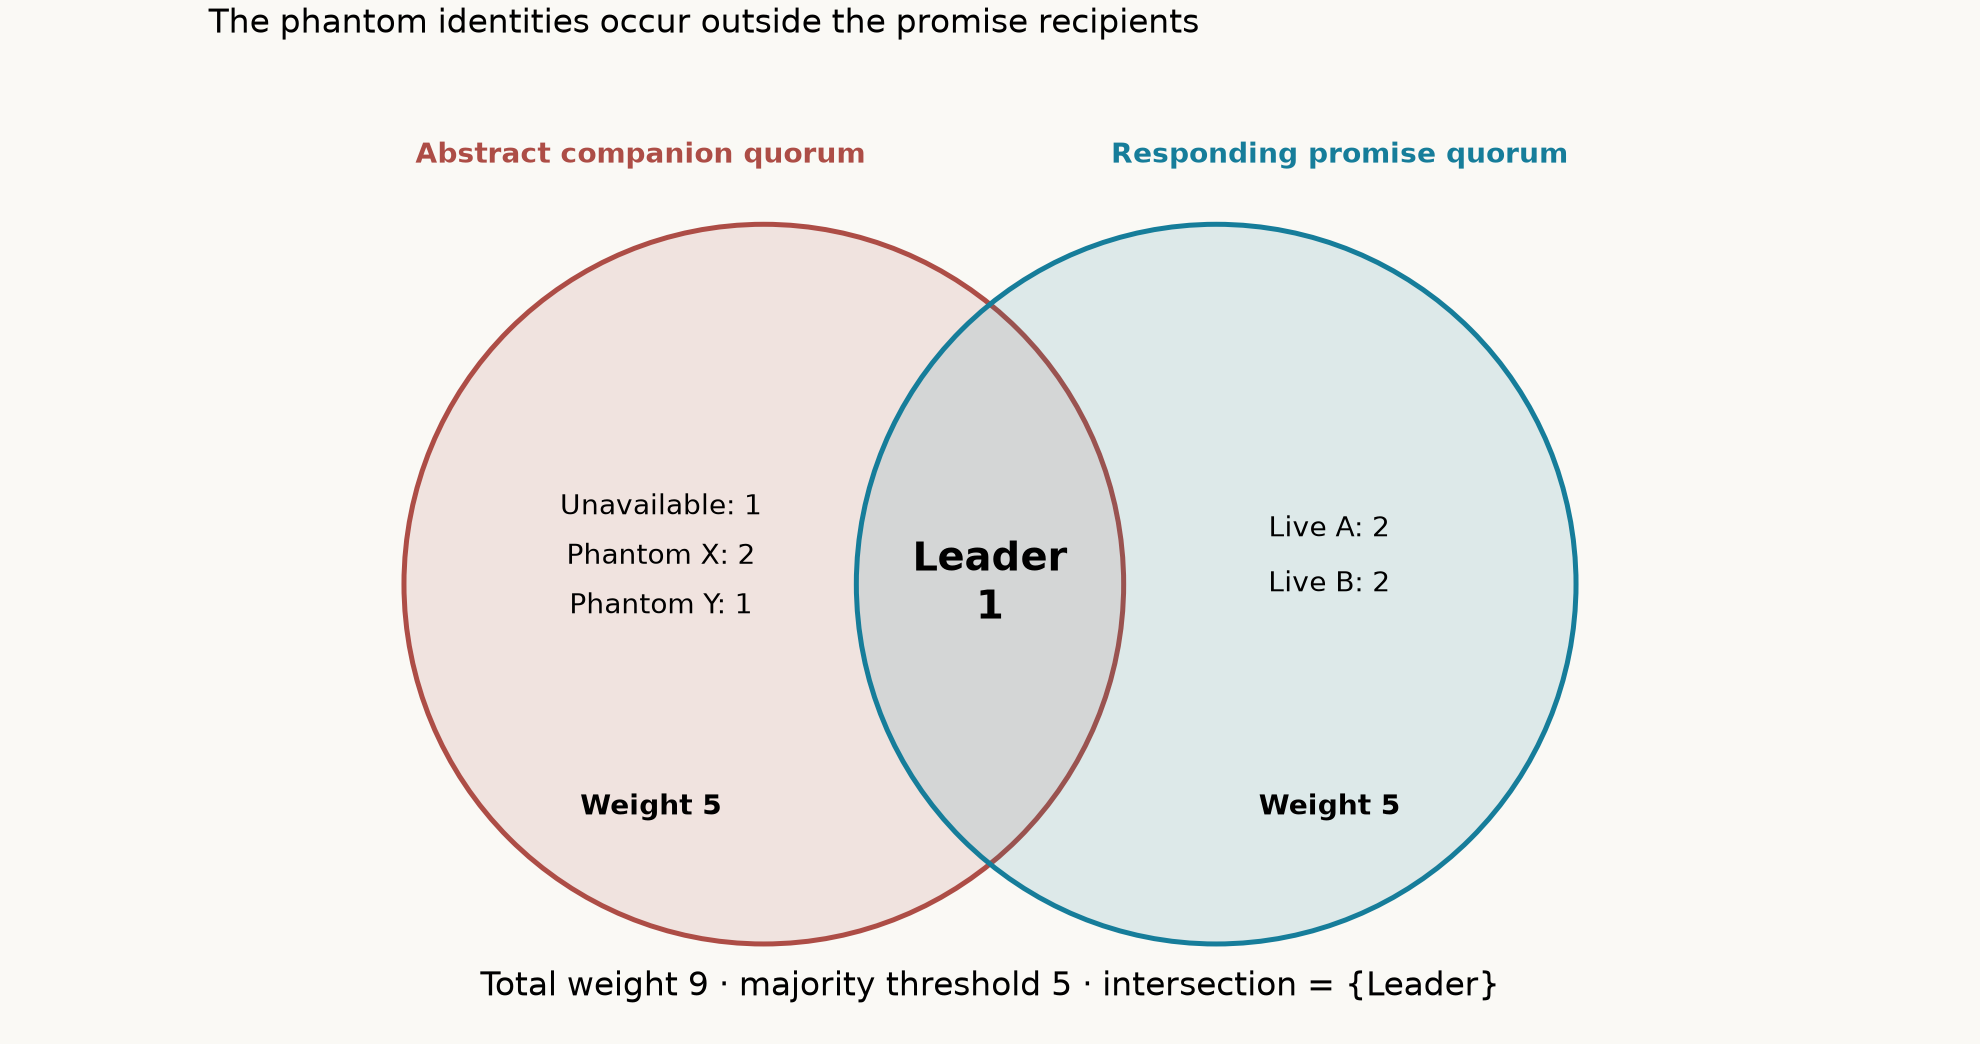
\includegraphics[width=0.94\textwidth]{diagrams/weighted-quorum-witness.png}
\caption{Sharp phantom-mass example, generated by the Python checker. The preparing quorum uses available identities; its abstract companion includes fresh identities. Both have weight five out of nine and intersect only at the leader. Fresh identities do not supply message receipts.}
\label{fig:phantom}
\end{figure*}

\subsection{Equal total mass and datacentre resilience}
Equal total mass alone does not imply cross-era intersection. For $(1,2,1,2)\to(2,1,2,1)$ on $(A,B,C,D)$, $\{B,D\}$ is an old majority and $\{A,C\}$ a disjoint new majority. The solver instead returns
\[
(1,2,1,2)\to(2,2,1,2)\to(2,2,2,2)
\]
\[
\to(2,1,2,2)\to(2,1,2,1).
\]
Each of these four boundaries is safe. For datacentres holding $(A,B)$ and $(C,D)$ at weights $(1,1,2,2)$, loss of the second leaves mass two out of six; loss of the first leaves mass four. This asymmetry can be deliberate. Four unit voters split two per datacentre can use flexible phase-two quorums of two with phase-one quorums of three: local decisions and local leader election have different availability conditions. The solver's guarantee is for strict weighted majorities; a flexible quorum policy must pass the core's role-specific intersection gates separately.

\subsection{Executable interface and validation}
The dependency-free Rust module \path{src/solver.rs} exposes \path{solve} and \path{solve_replacement}. Results are ordered \path{EraStep} batches with the resulting configurations; the target era is ignored and eras advance from the committed source. A request without an available majority at either endpoint returns the available and total masses. The replacement entrypoint prefers the complete standard schedule when its intermediate configurations remain available and its endpoint matches; otherwise it invokes the general constructor. The three-unit-voter schedule has two batches and the five-unit-voter schedule has all six batches in Table~\ref{tab:weights}. Replanning uses the current committed configuration.

The command-line binary \path{reconfiguration-solver} accepts ordered \code{id:weight} lists, a target list or \code{--replace old:new}, and an available-identity list. Each output row states the batch, resulting weights and available mass. State acquisition precedes promotion. If a different leader is needed, the existing \path{next_view_selecting} and administrative view-change input select a later ballot directly; the ordinary quorum-backed view-change exchange still establishes leadership. A local era increment does not constitute that exchange.

Rust property tests sample arbitrary six-identity source and target weights in $\{0,1,2\}$ subject to available majorities, replay every batch, and check every boundary with the exhaustive quorum gate. Deterministic tests cover the equal-mass counterexample, all 36 original-leader/failed-host combinations for two nodes in each of three datacentres, exact standard schedule lengths, and disjoint 16-member endpoints. The protocol test drives all 36 unit-weight cases through leader timeout when required, reincarnation announcements, view changes and client commits. Datacentre-loss assertions describe the restored uniform configuration, not every intermediate schedule.

The independent Python checker and generated figures are in \path{research/weighted-reachability/}. Its exhaustive run covers 310,007 symmetry representatives through ten identities (14,541,815 labelled profiles) and 774,159 endpoint-pair representatives through six identities (3,939,756 labelled pairs), with zero failed checks. These finite counts are computational evidence; the general claim rests on the proof above and the separately stated Lean theorems. Reproduce the Rust checks with \code{cargo test --test reconfiguration\_solver --test reconfiguration\_stepwise}, and the proof checks with \code{lake build} and \code{python3 check\_axioms.py} in the Lean project. The Leanstral driver's \code{check} command also accepts the module without proof holes or compiled-decision shortcuts.

\begin{thebibliography}{10}
\bibitem{fuse-paxos} L. Lamport, ``Paxos made simple,'' 2001. [Online]. Available: \url{https://www.microsoft.com/en-us/research/wp-content/uploads/2014/03/paxos-simple.pdf}
\bibitem{vr} B. M. Oki and B. H. Liskov, ``Viewstamped replication: A new primary copy method to support highly-available distributed systems,'' in \emph{ACM PODC}, 1988, pp. 8--17.
\bibitem{vrr} B. Liskov and J. Cowling, ``Viewstamped replication revisited,'' MIT CSAIL, Tech. Rep. MIT-CSAIL-TR-2012-021, 2012. [Online]. Available: \url{https://hdl.handle.net/1721.1/71763}
\bibitem{diskless} E. Michael, D. R. K. Ports, N. Kr. Sharma, and A. Szekeres, ``Providing stable storage for the diskless crash-recovery failure model,'' University of Washington, Tech. Rep. UW-CSE-16-08-02, Aug. 25, 2016. [Online]. Available: \url{https://syslab.cs.washington.edu/papers/diskless-tr16.pdf}
\bibitem{turner} D. Turner, ``Unbounded pipelining in dynamically reconfigurable Paxos clusters,'' revision 1A9DBA37, Aug. 14, 2017. [Online]. Available: \url{https://github.com/DaveCTurner/paxos-membership}. The proof artifact includes the consulted PDF and its digest.
\bibitem{motivation} S. Massey, ``Viewstamped replication revisited,'' Aug. 12, 2026. [Online]. Available: \url{https://simbo1905.wordpress.com/2026/08/12/viewstamped-replication-revisited/}
\bibitem{corfu} M. Balakrishnan, D. Malkhi, J. D. Davis, V. Prabhakaran, M. Wei, and T. Wobber, ``CORFU: A Distributed Shared Log,'' \emph{ACM Trans. Comput. Syst.}, vol. 31, no. 4, Art. 10, Dec. 2013, doi: \href{https://doi.org/10.1145/2535930}{10.1145/2535930}.
\bibitem{zookeeper} P. Hunt, M. Konar, F. P. Junqueira, and B. Reed, ``ZooKeeper: Wait-free coordination for Internet-scale systems,'' in \emph{USENIX ATC}, 2010. [Online]. Available: \url{https://www.usenix.org/events/usenix10/tech/full_papers/Hunt.pdf}
\bibitem{etcd-guarantees} etcd authors, ``etcd API guarantees,'' documentation v3.6, accessed Sep. 11, 2026. [Online]. Available: \url{https://etcd.io/docs/v3.6/learning/api_guarantees/}
\bibitem{etcd-hardware} etcd authors, ``Hardware recommendations,'' documentation v3.6, accessed Sep. 11, 2026. [Online]. Available: \url{https://etcd.io/docs/v3.6/op-guide/hardware/}
\bibitem{etcd-embed} etcd authors, ``Embedding etcd in a Go application,'' documentation v3.6, accessed Sep. 11, 2026. [Online]. Available: \url{https://etcd.io/docs/v3.6/dev-guide/golang_embed_pkg/}
\bibitem{artifact} S. Massey, ``uVRR proof artifact,'' commit 352b0bf, 2026. [Online]. Available: \url{https://github.com/lua-lunet/uvrr-core/tree/352b0bf/formal/uvrr-lean}
\bibitem{lean4} L. de Moura and S. Ullrich, ``The Lean 4 theorem prover and programming language,'' in \emph{Automated Deduction -- CADE 28}, 2021, pp. 625--635, doi: \href{https://doi.org/10.1007/978-3-030-79876-5_37}{10.1007/978-3-030-79876-5\_37}.
\end{thebibliography}
\end{document}
